%template1.tex
%The following LaTeX source file represents the simplest kind of slide presentation; no overlays, no included graphics. Substitute your favorite style for ``pascal''. To create the PDF file template1.pdf, (1) be sure to use the prosper class, then (2) execute the command latex template1.tex, and (3) the command dvipdf template1.dvi.

%%%%%%%%%%%%%%%%%%%%%%%%%%%%%%% template1.tex %%%%%%%%%%%%%%%%%%%%%%%%%%%%%%%%%%%
\documentclass[a4paper,blends,pdf,colorBG,slideColor]{prosper}
% definitions for slides for CSC544
% Lutz Hamel, (c) 2007

\hypersetup{pdfpagemode=FullScreen}

\usepackage{amssymb}
\usepackage{latexsym}
\usepackage{amsmath}
%\usepackage[usenames]{color}
\usepackage{xypic}


\newcommand{\term}[1]{\ensuremath{\mbox{\bf #1}}}
\newcommand{\nonterm}[1]{\ensuremath{\mbox{#1}}}
\newcommand{\ifstmt}[3]{\ensuremath{{\bf if}\; {#1}\;{\bf then}\;{#2}\;{\bf else}\;{#3}\;\term{end}}}
\newcommand{\whilestmt}[2]{\ensuremath{{\bf while}\; {#1}\;{\bf do}\;{#2}\; \term{end}}}
\newcommand{\funcstmt}[3]{\ensuremath{{\bf fun}\; {#1}\; {\bf is}\; {#2} \; {\bf return}\; {#3}}}
\newcommand{\syntaxset}[1]{\ensuremath{\mbox{\bf #1}}}
\newcommand{\orbar}{\;|\;}
\newcommand{\bs}[1]{\begin{slide}{#1}\ptsize{8}}
\newcommand{\es}{\end{slide}}
\newcommand{\co}{\,\colon\;}
\newcommand{\pair}[2]{\ensuremath{\langle {#1}, {#2} \rangle}}
\newcommand{\encode}[1]{\ensuremath{\langle {#1} \rangle}}
\newcommand{\mytab}{\makebox[.15in]{}}
%\newcommand{\abs}[1]{{\mid{#1}\mid}}
\newcommand{\abs}[1]{{|{#1}|}}
\newcommand{\ol}[1]{\overline{#1}}

\newcommand{\qaccept}{\ensuremath{q_{\mbox{\tiny accept}}}}
\newcommand{\qreject}{\ensuremath{q_{\mbox{\tiny reject}}}}
\newcommand{\accept}{{\em accept}}
\newcommand{\reject}{{\em reject}}

\newcommand{\machine}[1]{
	\begin{quote}
	{#1}
	\end{quote}
	}

\newcommand{\fdef}[1]{
	\begin{center}
	\fbox{
	\begin{minipage}{3.5in}
	{\bf Definition:}
	{#1}
	\end{minipage}
	}
	\end{center}
	}

\newcommand{\ftheorem}[1]{
	\begin{center}
	\fbox{
	\begin{minipage}{3.5in}
	{\bf Theorem:}
	{#1}
	\end{minipage}
	}
	\end{center}
	}

\newcommand{\flemma}[1]{
	\begin{center}
	\fbox{
	\begin{minipage}{3.5in}
	{\bf Lemma:}
	{#1}
	\end{minipage}
	}
	\end{center}
	}


\newcommand{\fframe}[1]{
	\begin{center}
	\fbox{
	\begin{minipage}{3.5in}
	{#1}
	\end{minipage}
	}
	\end{center}
	}

\newcommand{\nframe}[1]{
	\begin{center}
	\begin{minipage}{3.5in}
	{#1}
	\end{minipage}
	\end{center}
	}

\begin{document}

\bs{Nondeterministic Time Complexity}
\fdef{Let $N$ be a nondeterministic Turing machine that is a decider.  The {\bf\em running time} of $N$ is the function $f\co{\mathbb N} \rightarrow{\mathbb N}$, where $f(n)$ is the maximum number of steps that $N$ uses on {\em any branch of its computation} on any input of length $n$.}

\begin{center}
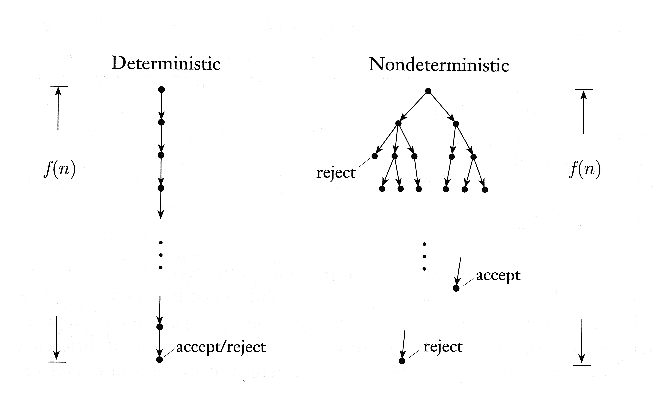
\includegraphics[height=40mm]{images/ntime.eps}
\end{center}
\es

\bs{Some Theorems}

\fframe{{\bf Theorem:} Let $t(n)$ be a function, where $t(n) \ge n$, then every $t(n)$ time multitape
Turing machine has an equivalent $O(t^2(n))$ time single tape Turing machine.}

{\bf Proof Sketch:} It is possible to show that simulating each of the $t(n)$ computation steps of the multitape machine
on a single tape machine takes at most $O(t(n))$ steps.  Therefore, to simulate the complete multitape
computation on a single tape machine will take $t(n)\times O(t(n)) = O(t^2(n))$ steps.

{\bf Observation:} Moving a computation from a multi-tape machine to a single-tape machine incurs an polynomial runtime penalty.
\es


\bs{Some Theorems}

\fframe{{\bf Theorem:} Let $t(n)$ be a function where $t(n)\ge 0$, then every $t(n)$ time nondeterministic single-tape Turing machine has an equivalent $2^{O(t(n))}$ time deterministic single-tape Turing machine.}

\scriptsize
{\bf Proof Sketch:} Recall that simulating a nondeterministic Turing machine with a deterministic Turing machine can be viewed as searching the tree of nondeterministic computations for accepting states.
Since the nondeterministic TM is a $O(t(n))$ time machine, the path from the root to a leaf node is bounded by $O(t(n))$ steps.  There are at most $b^{O(t(n))}$ leaf nodes in the tree.  Therefore we need to search
\[
O(t(n))\times b^{O(t(n))} = b^{O(t(n))} = 2^{O(t(n))} 
\]
positions.  Now, if we use a multi-tape deterministic TM, then we incur a polynomial penalty,
\[
(2^{O(t(n))})^2 = 2^{O(t(n)) + O(t(n))} = 2^{2O(t(n))} = 2^{O(t(n))}.
\]
Searching the tree for an accepting state is an exponential operation bounded by $2^{O(t(n))}$ steps.

{\bf Observation:} Moving a computation from a nondeterministic machine to a deterministic machine incurs an exponential runtime penalty.
\es

\bs{Time Complexity Classes}
\fdef{Let $t\co {\mathbb N} \rightarrow {\mathbb R}^+$ be a function.  Define the {\bf\em time complexity class},
$TIME(t(n))$, to be the collection of all languages that are decidable by an $O(t(n))$ time Turing machine, formally,
\[
TIME(t(n)) = \{ L | \mbox{$L$ is a language decided by an $O(t(n))$ time TM\}}.
\]}

{\bf Example:} Consider $A=\{0^k 1^k | k \ge 0\}$.  We have shown that $A \in TIME(n^2)$ and also
that $A \in TIME(n)$.

{\bf Observation:} Notice that the same language can be a member of many time complexity classes depending on how clever we are with devising algorithms.

{\bf Observation:} Perhaps this classification scheme is too fine grained, it does not capture the fundamental complexity differences between languages.
\es

\bs{The Class $P$}
Note that the difference between the algorithms of deciding the language $A$ are polynomial differences, that is, $O(n^2)$ versus $O(n)$.

In general we can say that all reasonable deterministic  computational models are {\bf\em polynomially equivalent} -- that is, any one of them can simulate another with only a polynomial increase in running time.

Compare this to algorithms that run efficiently on nondeterministic machines; simulating these algorithms on deterministic machines would incur an exponential increase in running time.

This motivates the polynomial time class $P$.

\fdef{$P$ is the class of languages that are decidable in polynomial time on a deterministic Turing machine,
\[
P = \bigcup_k TIME(n^k), \mbox{ for $k \ge 0$.}
\]}
\es


\bs{The Class $P$}
The class $P$ is interesting because:
\begin{itemize}
\item $P$ is invariant for all models of computation that are polynomially equivalent to the deterministic single-tape Turing machine.
\item $P$ roughly corresponds to the class of problems that are realistically solvable on a computer (i.e., the computer is a reasonable deterministic computational model).
\end{itemize}

{\bf Example:} Note that with this definition our language $A=\{0^k 1^k | k \ge 0\}$ is clearly a member
of $P$ regardless of which exact algorithm we use to decide it.
\es

\bs{$PATH \in P$}
{\small
\fframe{{\bf Theorem:} $PATH \in P$, where $PATH = \{ \encode{G,s,t} | $ $G$ is a directed graph that has a directed path from node $s$ to node $t$ $\}$.}

\scriptsize
{\bf Proof:}  A brute force search for the path does not work, since such an algorithm will run in exponential time (compare to the tree searching when simulating a nondeterministic TM).

However, we can be clever and implement an incremental search.
\begin{quote}
$M$ = "On input $\encode{G,s,t}$:
\begin{itemize}
\item[1.] Place a mark on node $s$.
\item[2.] Repeat the following until no additional nodes are marked:
\begin{itemize}
\item[3.] Scan all edges of $G$.  If an edge $(a,b)$ is found going from a marked node $a$ to
an unmarked node $b$, mark node $b$.
\end{itemize}
\item[4.] If $t$ is marked, \accept; otherwise, \reject."
\end{itemize}
\end{quote}
Analysis. It is clear that stages 1 and 4 run in constant time (or $O(n)$ where $n = |\encode{G,s,t}|$).
Stage 3 runs at most $m$ times where $m$ is the number of nodes in the graph.  Considering that we have to scan the representation of $G$ every time through the loop we obtain $O(m\times n)$ computation
steps.  Now considering that $m = \frac{1}{k}\times n$ with $k=1,2,\ldots$, that is, $m$ is a fraction of the total representation.
This gives us an overall complexity of the algorithm of 
\[
O(m\times n) = O( \frac{1}{k}\times n \times n) = O(n^2).
\]
Thus $PATH \in P$. $\Box$
}
\es


\bs{$CFL\in P$}
\fframe{{\bf Theorem:} Every context-free language is in $P$.}

{\bf Proof:} The brute force method does not work, have to search the full derivation tree for all possible derivation,
we can use the Chomsky normal form for this - but this is an exponential time problem.

However, we can use dynamic programming where we store previously computed partial solutions.  This is
how real parsing algorithms work.  Time complexity $O(n^3)$.$\Box$

\es

\bs{Class $NP$}
This is the class of problems that either have as of yet unknown polynomial solutions or are intrinsically difficult (simply do not have a polynomial solution).

\fdef{We define the {\bf\em nondeterministic time complexity class} NTIME as follows,
$
NTIME(t(n)) = \{ L | L$ is a language decided by an $O(t(n))$ time nondeterministic TM$\}$.
}

\fdef{
\[
NP = \bigcup_k NTIME(n^k), \mbox{ for $k \ge 0$}.
\]}
\es

\end{document}
%%%%%%%%%%%%%%%%%%%%%%%%%%% end of template1.tex %%%%%%%%%%%%%%%%%%%%%%%%%%%%%%%%

